% !TeX spellcheck = ru_RU
% !TEX root = bfs_lodygin.tex

\section{Эксперимент}

В данном разделе предлагается рассмотреть результаты экспериментального исследования реализованного алгоритма обхода графа в ширину. Основная задача: выявить зависимость производительности алгоритма от входных параметров графа и количества асинхронных потоков, обрабатывающих данный алгоритм.

\subsection{Условия эксперимента}
Для экспериментов использовалась рабочая станция с процессором Intel Core i5-10300H с тактовой частотой 2.50GHz, RAM DDR4 объемом 8гб под управлением OC Windows 10.

\subsection{Исследовательские вопросы }

\begin{itemize}
\item[\textbf{RQ1:}] При каких параметрах графа выгоднее использовать параллельную версию алгоритма, а при каких последовательную?
\item[\textbf{RQ2:}] Использование какого количества потоков даёт наибольший выигрыш в производительности и почему?
\end{itemize}


\subsection{Метрики}
В качестве метрик производительности используется время, требуемое на завершение алгоритма. Показатели времени получены с помощью библиотеки \texttt{BenchmarkDotNet v0.13.5}\footnote{Репозиторий библиотеки \texttt{BenchmarkDotNet}: \url{https://github.com/dotnet/BenchmarkDotNet} (дата доступа:   \DTMdate{2023-05-21}).}. Для замеров были выбраны стандартные настройки по \enquote{прогреву} и количеству итераций для измерений.

Для анализа алгоритма было решено воспользоваться собственным генератором графов нужного размера с нужной плотностью. Данный подход позволяет минимизировать влияние разницы прочих параметров на исследуемый, следовательно результаты, полученные в таком исследовании, позволят точнее выявить необходимые зависимости, нежели при использовании уже существующих графов. Генератор принимает на вход количество вершин в графе и параметр \texttt{density} типа \texttt{float}, отвечающий за плотность графа. По количеству заданных вершин создаётся двумерный массив, ячейки которого заполняются следующим образом. Если параметр плотности графа меньше $0.5$, все ячейки массива заполняются \texttt{Option.None}, затем с помощью цикла в случайных ячейки массива заносятся сгенерированные случайные числа \texttt{int}, обёрнутые в тип \texttt{Option}, пока не будет достигнута необходимая плотность. В противном случае, массив полностью заполняется случайными числами типа \texttt{int}, обёрнутыми в тип \texttt{Option}, а в случайные ячейки заносятся \texttt{Option.None}, пока опять же таки не будет достигнута необходимая плотность. 

\subsection{Результаты}

Входные параметры:
 \begin{enumerate}
 \item  \texttt{Vertices} --- количество вершин в графе; 
 \item  \texttt{Density} --- плотность графа;
 \item \texttt{parallelMult} --- уровень распараллеливания функции умножения, каждый уровень увеличивает число подзадач в 4 раза;
  \item \texttt{parallelAdd} --- уровень распараллеливания функции сложения, каждый уровень увеличивает число подзадач в 2 раза.
\end{enumerate}

Результаты замеров:
\begin{enumerate}
\item  \texttt{Time} --- результат измерений в мс (за исключением таблицы~\ref{bfscomparison}, где время измерений указано в микросекундах и таблицы~\ref{bfsmaxgraph}, где время указано в секундах);
\end{enumerate}

Замеры проводились начиная от очень малых графов (10 вершин), заканчивая графами с 5000 вершинами. Дополнительно были исследованы графы с 10000 вершинами, но очень малой плотности. Выбор максимального размера графа связан с ограничением оперативной памяти системы, на которой производились вычисления.

В таблице~\ref{bfs0} представлены результаты замеров времени работы последовательного алгоритма при различных входных параметрах графа. Из данной таблицы видно, что время работы алгоритма возрастает с увеличением плотности графа, а затем, когда граф достигает плотности $0.5$ начинает снижаться. Не трудно догадаться, что при высокой плотности графа уменьшается количество шагов алгоритма, необходимых для его завершения, так как за каждый шаг будет осуществляться переход в большее количество смежных вершин, следовательно общее время работы уменьшается.

\begin{table}[h]
\centering
    \caption{Производительность последовательного алгоритма обхода графов в ширину.}
    \rowcolors{2}{black!2}{black!10}
    \scalebox{0.7}{
    \begin{tabular}{| a | r | r | a | r | r |}
    \hline
        \textsc{Vertices} & \textsc{Density} & \textsc{Time $\pm$ Error} &
         \textsc{Vertices} & \textsc{Density} & \textsc{Time $\pm$ Error} \\ 
        \hline
        500 & 0.1 & $17 \pm 0.1$ & 2500 & 0.1 & $429 \pm 2$  \\ 
        500 & 0.3 & $33 \pm 0.3$ & 2500 & 0.3 & $860 \pm 3$ \\
        500 & 0.5 & $44 \pm 0.2$ & 2500 & 0.5 & $1091 \pm 8$ \\
        500 & 0.7 & $42 \pm 0.2$ & 2500 & 0.7 & $1095 \pm 3$  \\ 
        500 & 0.9 & $36 \pm 0.2$ & 2500 & 0.9 & $980 \pm 4$  \\ 
        
        1000 & 0.1 & $68 \pm 0.4$ & 5000 & 0.1 & $1717 \pm 3$ \\ 
        1000 & 0.3 & $137 \pm 0.6$ & 5000 & 0.3 & $3531 \pm 20$ \\
        1000 & 0.5 & $182 \pm 1.1$ & 5000 & 0.5 & $4426 \pm 23$ \\
        1000 & 0.7 & $179 \pm 1.2$ & 5000 & 0.7 & $4421 \pm 9$ \\ 
        1000 & 0.9 & $158 \pm 0.3$ & 5000 & 0.9 & $3984 \pm 14$ \\ 
    \hline    
    \end{tabular}%
    }
    \label{bfs0}
\end{table}

В таблице~\ref{bfsparallel} приведены результаты замеров времени работы параллельного алгоритма обхода графа при различных параметрах. Для удобства, при каждом параметре плотности графа взята наилучшая скорость среди всех параллельных версий алгоритма. Из полученных результатов можно заметить, что при увеличении размеров графа, наиболее оптимальное количество подзадач для параллельных вычислений выравнивается к 16 для функции умножения. Стоить отметить, что на достаточно больших графах, при одном и том же уровне распараллеливания функции умножения, влияние распараллеливания функции сложения становится не столь существенным, любая из комбинаций даёт один и тот же результат по времени в пределах погрешности (таблица~\ref{parallelAddvsparallelMult}). Связано это с тем, что наибольший процент времени выделяется под функцию умножения, как наиболее затратную по ресурсам.

\begin{table}[H]
\centering
    \caption{Производительность параллельного алгоритма обхода графов в ширину (лучшие данные по метрике). Графа \texttt{SpeedUp} показывает отношение скорости работы параллельной версии алгоритма к скорости работы последовательной версии. }
    \rowcolors{2}{black!2}{black!10}
    \scalebox{0.7}{
    \begin{tabular}{| a | r | r | r | r | r |}
    \hline
        \textsc{Vertices} & \textsc{Density} & \textsc{parallelMult} & \textsc{parallelAdd} & \textsc{SpeedUp}\\
        \hline
        500 & 0.1 & 2 & 1 & 0.53\\ 
        500 & 0.3 & 1 & 1 & 0.57\\ 
        500 & 0.5 & 1 & 1 & 0.56\\ 
        500 & 0.7 & 1 & 2 & 0.62\\
        500 & 0.9 & 2 & 2 & 0.64\\        
        1000 & 0.1 & 1 & 1 & 0.54\\ 
        1000 & 0.3 & 1 & 1 & 0.53\\ 
        1000 & 0.5 & 1 & 1 & 0.5\\
        1000 & 0.7 & 1 & 2 & 0.55\\ 
        1000 & 0.9 & 1 & 3 & 0.57\\ 
        2500 & 0.1 & 2 & 3 & 0.56 \\
        2500 & 0.3 & 2 & 3 & 0.54 \\
        2500 & 0.5 & 2 & 1 & 0.53 \\
        2500 & 0.7 & 2 & 3 & 0.59\\
        2500 & 0.9 & 2 & 1 & 0.6  \\ 
        5000 & 0.1 & 2 & 1 & 0.56 \\ 
        5000 & 0.3 & 2 & 3 & 0.51 \\
        5000 & 0.5 & 2 & 1 & 0.53 \\
        5000 & 0.7 & 2 & 3 & 0.59 \\ 
        5000 & 0.9 & 2 & 1 & 0.58 \\ 
    \hline    
    \end{tabular}%
    }
    \label{bfsparallel}
\end{table}

\begin{table}[h]
\centering
    \caption{Сравнение влияния уровня распараллеливания функции умножения и уровня распараллеливания функции сложения на графе с 5000 вершинами.}
    \rowcolors{2}{black!2}{black!10}
    \scalebox{0.7}{
    \begin{tabular}{| a | r | r | r | r |}
    \hline
        \textsc{Vertices} & \textsc{Density} & \textsc{parallelMult} & \textsc{parallelAdd} & \textsc{Time $\pm$ Error}\\ 
        \hline
        5000 & 0.1 & 1 & 1 & $1411 \pm 10$  \\ 
        5000 & 0.1 & 1 & 2 & $1401 \pm 12$  \\
        5000 & 0.1 & 1 & 3 & $1409 \pm 9$  \\
        5000 & 0.1 & 2 & 1 & $970 \pm 19$  \\
        5000 & 0.1 & 2 & 2 & $998 \pm 19$  \\
        5000 & 0.1 & 2 & 3 & $980 \pm 19$  \\
        5000 & 0.1 & 3 & 1 & $1126 \pm 21$  \\
        5000 & 0.1 & 3 & 2 & $1138 \pm 23$  \\
        5000 & 0.1 & 3 & 3 & $1151 \pm 18$  \\
    \hline    
    \end{tabular}%
    }
    \label{parallelAddvsparallelMult}
\end{table}


Так как на всех параметрах графа параллельная версия алгоритма обходила по производительности последовательную, было решено произвести дополнительные замеры при графах с меньшим количеством вершин (таблица~\ref{bfscomparison}). Выяснилось, что при таких размерах графа последовательная версия работает значительно быстрее, чем параллельная.

\begin{table}[h]
\centering
    \caption{Сравнение производительности параллельного и обычного Bfs на графах с 10 вершинами. Графа \texttt{SpeedUp} показывает отношение скорости работы параллельной версии алгоритма к скорости работы последовательной версии.}
    \rowcolors{2}{black!2}{black!10}
    \scalebox{0.7}{
    \begin{tabular}{| a | r | r | r | r |}
    \hline
        \textsc{Vertices} & \textsc{Density} & \textsc{TimeBfs $\pm$ Error} & \textsc{TimeParallelBfs $\pm$ Error} & \textsc{SpeedUp}\\
        \hline
        10 & 0.1 & $15.00 \pm 0.03$ & $53 \pm 0.2$ & 3.5 \\ 
        10 & 0.3 & $20 \pm 0.4$ & $78 \pm 0.3$ & 3.9 \\
        10 & 0.5 & $32 \pm 0.3$ & $124 \pm 1.3$ & 3.8 \\
        10 & 0.7 & $27 \pm 0.5$ & $60 \pm 0.4$ & 2.2 \\
        10 & 0.9 & $25 \pm 0.6$ & $44 \pm 0.4$ & 1.76\\ 
    \hline    
    \end{tabular}%
    }
    \label{bfscomparison}
\end{table}

Однако, уже на графах с 50 вершинами параллельная версия догоняет и начинает опережать последовательную версию по производительности.

\begin{table}[h]
\centering
    \caption{Сравнение производительности параллельного и обычного Bfs на графах с 50 вершинами. Графа \texttt{SpeedUp} показывает отношение скорости работы параллельной версии алгоритма к скорости работы последовательной версии.}
    \rowcolors{2}{black!2}{black!10}
    \scalebox{0.7}{
    \begin{tabular}{| a | r | r | r | r |}
    \hline
        \textsc{Vertices} & \textsc{Density} & \textsc{TimeBfs $\pm$ Error} & \textsc{TimeParallelBfs $\pm$ Error} & \textsc{SpeedUp}\\
        \hline
        50 & 0.1 & $293 \pm 6$ & $284 \pm 3$ & 0.97 \\ 
        50 & 0.3 & $372 \pm 7$ & $278 \pm 5$ & 0.74\\ 
        50 & 0.5 & $572 \pm 11$ & $614 \pm 9$ & 1.07\\
        50 & 0.7 & $438 \pm 7$ & $325 \pm 2$ & 0.74 \\
        50 & 0.9 & $416 \pm 8$ & $312 \pm 2$ & 0.75 \\ 
    \hline    
    \end{tabular}%
    }
    \label{bfscomparison}
\end{table}

Также, чтобы исследовать оптимальное разделение на подзадачи для функции умножения, как наиболее значимой для распараллеливания, были проведены замеры с теми же размерами и плотностями графа, но с использованием последовательной функции сложения. Результаты приведены в таблице~\ref{bfsparallelmult}.

\begin{table}[h]
\centering
    \caption{Производительность параллельного алгоритма обхода графов в ширину с использованием последовательной функции сложения веторов.}
    \rowcolors{2}{black!2}{black!10}
    \scalebox{0.6}{
    \begin{tabular}{| a | r | r | r | a | r | r | r |}
    \hline
        \textsc{Vertices} & \textsc{Density} & \textsc{parallelMult} & \textsc{Time $\pm$ Error} &
        \textsc{Vertices} & \textsc{Density} & \textsc{parallelMult} & \textsc{Time $\pm$ Error} \\ 
        \hline
        500 & 0.1 & 1 & $9,8 \pm 0.1$ & 2500 & 0.1 & 2 & $240 \pm 3$  \\ 
        500 & 0.3 & 1 & $19 \pm 0.4$ & 2500 & 0.3 & 2 & $470 \pm 9$ \\ 
        500 & 0.5 & 2 & $44 \pm 0.9$ & 2500 & 0.5 & 2 & $1004 \pm 19$ \\
        500 & 0.7 & 1 & $26 \pm 0.5$ & 2500 & 0.7 & 2 & $661 \pm 13$  \\
        500 & 0.9 & 2 & $24 \pm 0.4$ & 2500 & 0.9 & 2 & $620 \pm 12$  \\ 
        
        1000 & 0.1 & 1 & $36 \pm 0.5$ & 5000 & 0.1 & 2 & $923 \pm 18$ \\
        1000 & 0.3  & 1 & $72 \pm 1.4$ & 5000 & 0.3 & 2 & $1843 \pm 36$ \\
        1000 & 0.5  & 2 & $153 \pm 1.4$ & 5000 & 0.5 & 2 & $4143 \pm 78$ \\
        1000 & 0.7 & 1 & $98 \pm 1.6$ & 5000 & 0.7 & 2 & $2571 \pm 39$ \\ 
        1000 & 0.9 & 1 & $90 \pm 1.1$ & 5000 & 0.9 & 2 & $2372 \pm 41$ \\
    \hline    
    \end{tabular}%
    }
    \label{bfsparallelmult}
\end{table}

В ходе замеров было установлено, что при увеличении размеров графа, вне зависимости от плотности, время работы алгоритма при разделении на 16 подзадач для функции умножения хоть и больше, чем при работе с разделением на 64 подзадачи, но разрыв становится все меньше и меньше. Вследствие этого наблюдения, было решено произвести замеры для параллельных версий алгоритма для графов с 10000 вершинами, что являлось пределом допустимого значения количества вершин для обработки графа системой. Исследовались графы маленькой плотности с целью выяснить, сможет ли версия с 64 подзадачами обогнать по производительности версию с 16 подзадачами. Результаты приведены в таблице~\ref{bfsmaxgraph}.

\begin{table}[h]
\centering
    \caption{Сравнение производительности алгоритма обхода в ширину при распараллеливании на 16 и 64 подзадачи для функции умножения. Графа \texttt{SpeedUp} показывает отношение скорости работы алгоритма при 64 подзадачах к скорости работы при 16 подзадачах.}
    \rowcolors{2}{black!2}{black!10}
    \scalebox{0.6}{
    \begin{tabular}{| a | r | r | r | r | r |}
    \hline
        \textsc{Vertices} & \textsc{Density} & \textsc{parallelMult} & \textsc{Time $\pm$ Error} &
        \textsc{SpeedUp} \\ 
        \hline
        1000 & 0.1 & 2 & $0.0400 \pm 0.0003$ & 1.25 \\
        2500 & 0.1 & 2 & $0.240 \pm 0.002$ & 1.22 \\ 
        5000 & 0.1 & 2 & $0.90 \pm 0.03$ & 1.2 \\
        10000 & 0.1 & 2 & $4.00 \pm 0.07$ & 1.25 \\ 
    \hline    
    \end{tabular}%
    }
    \label{bfsmaxgraph}
\end{table}

Однако, как показало дополнительное измерение при графе с 10000 вершинами, по производительности всё так же лидирует распараллеливание на 16 подзадач, причём разрыв между скоростями вырос.

Результаты, полученные с помощью \texttt{BenchmarkDotNet} были проверены на адекватность с помощью библиотек \texttt{SciPy v1.10.1}\footnote{Сайт библиотеки \texttt{SciPy}: \url{https://scipy.org/} (дата доступа:   \DTMdate{2023-05-21}).}, \texttt{NumPy v1.24.3}\footnote{Сайт библиотеки \texttt{NumPy}: \url{https://numpy.org/} (дата доступа:\DTMdate{2023-05-21}).} и \texttt{Matplotlib v3.7.1}\footnote{Сайт библиотеки \texttt{MatPlotLib}: \url{https://matplotlib.org/} (дата доступа:   \DTMdate{2023-05-21}).} на языке \texttt{Python}. Например, рассмотрим данные, полученные при измерении производительности параллельной версии алгоритма на графе с 5000 вершинами плотности $0.9$ и уровнями распараллеливания parallelMult, равным двум, и parallelAdd, равным 1. Результаты замеров приведены в таблице~\ref{data}. 

\begin{table}[h]
\centering
    \caption{Замеры времени работы параллельной версии алгоритма на графе с 5000 вершинами плотности $0.9$. Функция умножения разделена на 16 подзадач, функция сложения на две. Время измерено в секундах.}
    \rowcolors{2}{black!2}{black!10}
    \scalebox{0.6}{
    \begin{tabular}{| a | r | r | r | r | r | r | r | r | r | r |}
    \hline
    N & 1 & 2 & 3 & 4 & 5 & 6 & 7 & 8 & 9 & 10 \\
    \hline
    Time & 2.4081 & 2.3506 & 2.3857 & 2.3383 & 2.2634 & 2.2931 & 2.2984 & 2.3895 & 2.2800 & 2.2899\\
    N & 11 & 12 & 13 & 14 & 15 & 16 & 17 & 18 & 19 & 20\\
    \hline
    Time & 2.3293 & 2.2977 & 2.2358 & 2.3113 & 2.4044 & 2.3317 & 2.3054 & 2.2614 & 2.4011 & 2.3421 \\
    \hline    
    \end{tabular}%
    }
    \label{data}
\end{table}

С помощью функций \texttt{scipy.stats.shapiro()} (тест Шапиро-Уилка) и \texttt{scipy.stats.normaltest()} (критерий согласия Пирсона) было проверено соответствие выборки нормальному распределению. Значение \texttt{pvalue} в результате проверок равнялось 0.36 (Шапиро) и 0.5 (Пирсон), что позволяет нам не отклонять \enquote{нулевую гипотезу} и считать полученные данные как нормальное распределение. Далее, с помощью функций \texttt{np.mean()} и \texttt{np.std()} были посчитаны среднее значение $Mean = 2.32586$ и стандартное отклонение $StdDev = 0.051$. Аналогичные результаты были получены и библиотекой \texttt{BenchmarkDotNet}: $Mean = 2.326$, $StdDev = 0.051$. При помощи \texttt{matplotlib.pyplot.hist()} была построена гистограмма (рисунок~\ref{fig:plot}) из полученной выборки.

\begin{figure}[H]
    \centering
    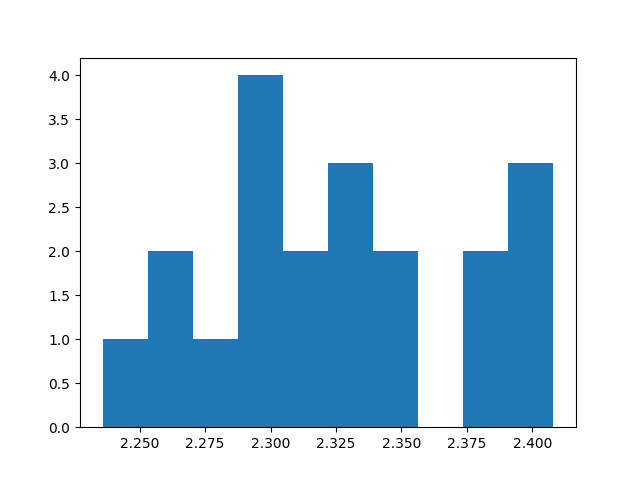
\includegraphics[width=\textwidth]{figures/plot.png}
    \caption{Гистограмма распределения времени работы алгоритма на графе из 5000 вершин плотности 0.9. Функция умножения разделена на 16 подзадач, функция сложения на две.}
    \label{fig:plot}
\end{figure}

\subsubsection{RQ1} Исходя из полученных данных, последовательная версия алгоритма работает быстрее параллельной только на очень малых графах (10 вершин), когда накладные расходы на выделение дополнительных потоков и их синхронизацию влияют сильнее, чем ускорение относительно последовательной версии. При входных графах от 50 вершин и более, параллельная версия даёт прирост к производительности вплоть до увеличения скорости работы алгоритма в 2 раза при любых параметрах плотности.
\subsubsection{RQ2} В ходе экспериментов было установлено, что использование разделения на 16 подзадач, начиная с определённых размеров графа (2500 вершин для системы, используемой при замерах), даёт максимальный прирост по производительности алгоритма обхода в ширину. Такой результат можно объяснить количеством ядер процессора. Система, на которой производились замеры имеет 4-х ядерный процессор \texttt{Intel Core i5-10300H}, вследствие чего количество независимых вычислителей равняется четырём. С другой стороны, данный процессор поддерживает технологию \texttt{Hyper-Threading}, позволяющую разделить одно ядро процессора на 2 отдельных логических процессора, работающих независимо. Таким образом наилучшая производительность наблюдается на 8 потоках, каждый из которых обрабатывает по 2 подзадачи. Польза от такого разделения влияет на конечное время работы алгоритма сильнее, чем затраты времени на выделение необходимых потоков и синхронизацию их работы.